%% CS-5187 term-project report in FSE format.
%% Course requirements (course page, "Deliverables", checked 2026-11-13):
%%   * ACM Primary Article Template, LaTeX `sigconf`, written in Overleaf
%%   * sections: motivation, technique, implementation, evaluation,
%%     related work, threats to validity
%%   * a signed contribution statement in the report
%%   * the PDF is submitted with the artifact
%%   * FSE reviews double-anonymously, so the report is anonymous: acmart's
%%     `anonymous` option, no names or affiliations in the source or the PDF,
%%     and no identifying links. The signed contribution statement with the
%%     authors' names is CONTRIBUTIONS.md in the replication package.
%%     `review` adds line numbers, as FSE submissions require.
\documentclass[sigconf,review,anonymous]{acmart}

%% Shared macros. Keep notation here so the paper cannot drift from itself.
%% Rule: every name, symbol and set used more than once gets a macro here.
\usepackage{amsmath}
\usepackage{booktabs}
\usepackage{xspace}
\usepackage{listings}
\usepackage{xcolor}
\usepackage{array}
\usepackage{pifont}
\usepackage{tikz}
\usetikzlibrary{arrows.meta,positioning,calc,fit,backgrounds}
\DeclareRobustCommand{\circled}[1]{\tikz[baseline=(c.base)]\node[circle,draw,inner sep=0.7pt,font=\tiny\bfseries] (c) {#1};}

% ---- project name (anonymised for review) ----
% Works for any CS-5187 project: a tool, a technique/method, or an empirical
% study. With no tool (e.g. a study), read \tool as "our study" and reword
% "We present \tool" -> "We study ...", "\tool records" -> "our method ...".
\newcommand{\tool}{\textsc{Graft}\xspace}   % the tool presented in this paper

% ---- notation (one macro per symbol; comment says what it means) ----
\newcommand{\Fz}{\ensuremath{F}\xspace}                  % the incumbent fuzzer of the engine under test
\newcommand{\Rengine}{\ensuremath{R}\xspace}                 % the reference engine that fuzzer compares against
\newcommand{\Voc}{\ensuremath{V_F}\xspace}               % function vocabulary of F
\newcommand{\VocR}{\ensuremath{V_R}\xspace}              % functions the reference engine implements
\newcommand{\Lit}{\ensuremath{L_F}\xspace}               % literal domain of F (integers and strings)
\newcommand{\Blind}{\ensuremath{B}\xspace}               % the blind spot of F
\newcommand{\imax}{\texttt{i64::MAX}\xspace}             % 9223372036854775807
\newcommand{\sql}[1]{\texttt{#1}}                        % inline SQL

% ---- research questions ----
\newcommand{\rqref}[1]{\textbf{RQ#1}\xspace}

% ---- results: one boxed, numbered claim per observation ----
\newcounter{observation}
\newsavebox{\obsbox}
\newenvironment{observation}
  {\refstepcounter{observation}\par\smallskip\noindent\begin{lrbox}{\obsbox}\begin{minipage}{0.95\linewidth}\textbf{Observation~\theobservation.}~}
  {\end{minipage}\end{lrbox}\fbox{\usebox{\obsbox}}\par\smallskip}

% ---- CS-5187 term-project FOCUS callouts (RED, on purpose) ----
% A red box that marks a part every term-project report MUST address:
%   Research Questions, Motivating Example, Workflow, Related Work,
%   Threats to Validity. The red is a study aid, not paper style -- once
%   you have written the section, DELETE its \focus{...} line (keep the
%   section). A finished report has zero \focus and zero \todo.
\newcommand{\focus}[1]{%
  \par\smallskip\noindent
  {\color{red}\rule{\linewidth}{0.6pt}}\par\nobreak\vspace{1pt}\noindent
  {\color{red}\ding{228}~\textbf{FOCUS --- graded, must address:}~\itshape #1}\par\nobreak\vspace{1pt}
  {\color{red}\rule{\linewidth}{0.6pt}}\par\smallskip}

% ---- editorial (all must be gone before submission; scripts/check.sh counts them) ----
\newcommand{\todo}[1]{\textcolor{red}{[TODO: #1]}}
\newcommand{\num}[1]{\textcolor{blue}{#1}}   % a number not yet measured by the final tool
\newcommand{\cmark}{\ding{51}}
\newcommand{\xmark}{\ding{55}}

\lstset{basicstyle=\ttfamily\footnotesize,columns=fullflexible,
        keepspaces=true,frame=single,framesep=2pt,xleftmargin=4pt,
        numbers=left,numberstyle=\tiny,numbersep=4pt}

% long \texttt words otherwise run into the margin
\setlength{\emergencystretch}{3em}


\setcopyright{none}
\acmConference[Term Project, FSE format]{Term project report in the format of the ACM International Conference on the Foundations of Software Engineering (FSE)}{November 2026}{Submitted for anonymous review}
\acmYear{2026}
\acmDOI{}   % a course report has no DOI; acmart otherwise prints a placeholder
\acmISBN{}
\settopmatter{printacmref=false}
\citestyle{acmauthoryear}

\begin{document}

\title[GRAFT]{GRAFT: Cross-Engine Bug-Report-Guided Fuzzing of a SQLite-Compatible Database}

\author{Anonymous Author(s)}
\affiliation{\institution{Anonymous Institution}\country{Anonymous}}

\begin{abstract}
A database engine must answer every statement or reject it with an error. Mature
engines check this with differential fuzzers that compare their answers against
a reference engine. Such a fuzzer cannot test a function it never generates, nor
judge one its reference engine lacks. Turso, a SQLite-compatible engine written
in Rust, runs such a fuzzer in continuous integration, yet the single statement
\sql{select LPAD('a', 9223372036854775807, 'b')} terminated the whole process.
We present \tool. It takes the shape of bug reports filed against a different
engine, DuckDB, refills their literals with boundary values, and runs them
against Turso together with a typed SQL generator. Its only oracle needs no
reference engine: one statement must not end the process. \tool found three
previously unknown defects in Turso's \sql{lpad}, \sql{rpad} and \sql{repeat}
functions. Each aborts the engine from one statement, and \tool regenerates each
from a recorded seed. Our patch for them exposed a fourth defect in the same
length check, which \tool did not find. Our two patches, which fix all four,
were merged upstream. None of Turso's own fuzzers can express any of the four,
since the three functions are absent from all of them. At an equal budget of
20{,}000 cases, mined reports and typed generation each reached both root causes
of the three defects, and drawing from both sources found the first defect at
case 101. The work taught us that reading an incumbent fuzzer's source is a cheap
and reliable way to decide where to test next.

\end{abstract}

\begin{CCSXML}
<ccs2012>
  <concept>
    <concept_id>10011007.10011074.10011099.10011102.10011103</concept_id>
    <concept_desc>Software and its engineering~Software testing and debugging</concept_desc>
    <concept_significance>500</concept_significance>
  </concept>
  <concept>
    <concept_id>10002951.10002952</concept_id>
    <concept_desc>Information systems~Data management systems</concept_desc>
    <concept_significance>300</concept_significance>
  </concept>
</ccs2012>
\end{CCSXML}
\ccsdesc[500]{Software and its engineering~Software testing and debugging}
\ccsdesc[300]{Information systems~Data management systems}

\keywords{fuzzing, database testing, SQL, bug reports, test generation, crash oracle}

\maketitle

\section{Motivation}
\label{sec:motivation}
\label{sec:intro}

Suppose a server process embeds a SQL engine and lets its users format reports
with \sql{lpad}, which pads a string to a requested width. A user types a width
of 9{,}223{,}372{,}036{,}854{,}775{,}807. The server should answer with an error
message. If the engine instead ends the process, every other user's session ends
with it. A database engine is trusted to be correct without being checked, so a
defect of this kind is caught by the engine's own tests or not at all.

Database engines are among the most heavily tested programs in practice.
Differential testing runs the same query on two engines and reports any
disagreement. Metamorphic oracles compare a query with an equivalent rewrite of
itself~\cite{rigger2020tlp,rigger2020norec}. Grammar-based generators produce
valid SQL at scale~\cite{zhong2020squirrel,liang2026sqlbull}. All of these tools
stop at two boundaries: the generator can only emit the functions and values it
was written to emit, and a differential oracle can only judge a feature that its
reference engine also implements. We focus on the defects that sit past those
two boundaries. Such defects are silent in a specific way: a fuzzer can run for
a year without reaching them, and the time it has already run says nothing about
how close it is.

\begin{figure*}[t]
\begin{lstlisting}[escapechar=@]
-- (a) Regression test added by the fix for DuckDB issue #27846
select LPAD('x', 10, '0'), LPAD('x', 4, '@\textcolor{black}{\ding{72}}@'), LPAD('x', 3, '@\textcolor{black}{\ding{72}}@ab'), RPAD('x', 3, '@\textcolor{black}{\ding{72}}@ab')
-- (b) The same shape with every literal replaced by a typed hole
select LPAD({s4}, {n0}, {s5}), LPAD({s6}, {n1}, {s7}), LPAD({s8}, {n2}, {s9}), RPAD({s10}, {n3}, {s11})
-- (c) Filled from a boundary pool at seed 0, then run on Turso b588fbdc6
select LPAD('', -9223372036854775808, 'abc'), LPAD('_', -128, '%'), LPAD('0', 9223372036854775807, 'abc'), RPAD('%', -128, 'ABC')
-- (d) Reduced to one statement
select LPAD('a', 9223372036854775807, 'b');
@\textit{memory allocation of 9223372036854775806 bytes failed}@      @$\leftarrow$ process aborts, exit status 134@
\end{lstlisting}
\caption{The motivating example. A regression test from another engine~(a),
templated~(b) and refilled with boundary values~(c), aborts Turso from one
statement~(d). The marker \ding{72} stands for a four-byte emoji in the original
test. Turso's own fuzzers cannot produce~(d): their 47-function vocabulary has
no \sql{lpad}, and their integers stop at 1{,}000{,}000.}
\label{fig:motivating}
\end{figure*}

Figure~\ref{fig:motivating} shows a real case. Turso~\cite{turso} is a
SQLite-compatible engine written in Rust. It runs its own differential fuzzer in
continuous integration: 41{,}205 lines of Rust that generate SQL and compare
Turso's answers with SQLite's. Yet the statement in Figure~\ref{fig:motivating}d
ended the process with exit status 134 (SIGABRT) in 2.28 seconds, where it should
have returned the engine's own error \emph{string or blob too big}. Turso's
fuzzer could never have produced it. Its vocabulary of 47 scalar functions does
not contain \sql{lpad}, and it draws integer literals only from
$[-1{,}000{,}000,\ 1{,}000{,}000]$~\cite{tursofuzzer}. Even if it had produced
the statement, SQLite has no \sql{lpad} to compare the answer against. None of
Turso's four libFuzzer targets or its differential fuzzer calls \sql{lpad},
\sql{rpad} or \sql{repeat}.

The closest prior work either chooses where to look from the grammar or reuses
known defects through static analysis. SQLBull starts generation from grammar
rules that a tester marks as feature-rich~\cite{liang2026sqlbull}.
Recurring-vulnerability detectors turn a known patch into a rule and search for
code that breaks it~\cite{cao2025vulpa,cao2025antman}. However, the first needs
someone to pick the starting rules, and the second needs the defect to recur in
shared or copied code. Turso and DuckDB share no code.

We present \tool, which finds defects in this region in four steps:
\begin{enumerate}
  \item It reads the incumbent fuzzer's source and lists the functions and
        values that fuzzer cannot generate (Section~\ref{sec:step-blind}).
  \item It mines closed, reproduced bug reports from a different engine and keeps
        each report's query as a template whose literals are typed holes
        (Section~\ref{sec:step-mine}).
  \item It fills those holes, and the output of a typed SQL generator, with
        boundary values, and runs every statement against the engine under test
        (Section~\ref{sec:step-run}).
  \item It flags any statement that ends the process, then reduces, re-checks and
        reports it (Section~\ref{sec:step-triage}).
\end{enumerate}

We ran \tool against Turso. It found three previously unknown defects in Turso's
string functions: \sql{lpad} and \sql{rpad} allocate their result before checking
its length, and \sql{repeat} also overflows its size computation. Our patch for
them moved the length check in front of the allocation, and that exposed a
fourth defect, which \tool did not find: the check counts characters against a
limit in bytes. Our two patches, which fix all four, were merged
upstream~\cite{turso11225,turso11259}. At an equal budget of 20{,}000 cases, the
mined reports and the typed generator each reached both root causes of the
three defects. The lesson we draw is a practical one: before spending compute on
a fuzzer, spend an hour reading the fuzzer that is already there.

\paragraph{Research contributions.}
\begin{itemize}
  \item We define the \emph{blind spot} of an incumbent fuzzer and show that it
        can be measured from that fuzzer's source (Section~\ref{sec:problem}).
  \item We present \tool, which fills the blind spot with the shapes of another
        engine's bug reports and with typed generation, and judges results with an
        oracle that needs no reference engine (Section~\ref{sec:technique}).
  \item We report three previously unknown defects in Turso found by \tool, each
        regenerated from a recorded seed, and a fourth that our fix exposed. All
        four are fixed upstream by our merged patches (Section~\ref{sec:rq1}).
  \item We measure what each input source contributes at an equal budget, and
        release the tool, the corpus and all data
        (Sections~\ref{sec:rq2} and~\ref{sec:data}).
\end{itemize}

The rest of this section gives the background the paper needs
(Section~\ref{sec:background}), states the problem precisely
(Section~\ref{sec:problem}), and explains why the obvious alternatives do not
solve it.

\subsection{Background}
\label{sec:background}

\paragraph{Turso.} Turso~\cite{turso} reimplements SQLite in Rust and aims to
accept the same SQL. Its shell, \texttt{tursodb}, reads statements on standard
input. Text and blob results are bounded by a constant,
\texttt{Value::MAX\_BLOB\_LENGTH}, of $10^9$ bytes. A statement whose result
would exceed it should fail with the error \emph{string or blob too big}, which
is SQLite error code~18. Rust aborts the process when an allocation fails and cannot be
recovered, so a size check that runs after the allocation is not a check at all.

\paragraph{Differential testing.} A \emph{differential oracle} runs one query on
two engines and reports a disagreement. It needs no knowledge of the correct
answer, but it needs a \emph{reference engine} that implements the same feature.
Turso's fuzzer uses SQLite as its reference engine. SQLite has no \sql{lpad},
\sql{rpad} or \sql{repeat}, so a disagreement on those functions cannot be
judged.

\paragraph{Crash oracle.} A \emph{crash oracle} reports a statement that ends the
engine's process, panics, reports an internal error or does not answer within a
time limit. It does not report a \emph{user error}, which is a statement the
engine rejects with a normal message, such as a syntax error or a documented
limit. A crash oracle needs no reference engine. It finds no wrong answer that
leaves the process running.

\paragraph{Bug reports as test material.} DuckDB maintainers add the label
\emph{reproduced} to an issue once they have confirmed it. A fix usually adds a
regression test that contains the query which triggered the issue. Such a query
is small, it was chosen by someone who understood the defect, and it tends to sit
in an awkward corner: an empty string, a multi-byte character, a value at the
edge of a type.

\paragraph{Literal and template.} We call a constant in a query, such as
\sql{10} or \sql{'x'}, a \emph{literal}. A \emph{template} is a query in which
every literal is replaced by a typed hole, such as \sql{\{n0\}} for an integer or
\sql{\{s4\}} for a string. Filling the holes gives a new query with the same
structure.

\subsection{The Blind Spot of an Incumbent Fuzzer}
\label{sec:problem}

Let \Fz be the fuzzer that already tests an engine~$E$, and let \Rengine be the
reference engine that \Fz compares against. We write \Voc for the set of SQL
functions that \Fz can emit, and \Lit for the literals it can emit: a range of
integers and a set of strings. We write \VocR for the functions that \Rengine
implements.

A statement $q$ is \emph{expressible} by \Fz if every function in $q$ is in \Voc
and every literal in $q$ is in \Lit. A statement is \emph{judgeable} if every
function in $q$ is in \VocR. The \emph{blind spot} of \Fz is
\begin{equation}
  \label{eq:blind}
  \Blind = \{\, q \mid q \text{ is not expressible by } \Fz
           \ \lor\ q \text{ is not judgeable against } \Rengine \,\}.
\end{equation}
\Fz never generates a statement outside its own vocabulary or literal domain,
however long it runs. A statement that \Fz does generate but cannot judge is
generated in vain. Both halves of~\eqref{eq:blind} are properties of the source
code of \Fz and \Rengine, so \Blind can be measured before any test runs.

\paragraph{Goal.} Find statements $q \in \Blind$ on which $E$ violates the crash
oracle, without a reference engine, and with each finding regenerated from a
recorded seed. We look for two things: which functions and values put a
statement in \Blind, and where to get statements in that region that are likely
to break $E$.

\subsection{Why the Obvious Alternatives Fall Short}

\paragraph{Why not widen the incumbent fuzzer instead?} Its maintainers could add
\sql{lpad} to \Voc and \imax to \Lit, and the defects in this paper would then be
within reach. But that needs someone to know which function and which value to
add. The blind spot is large: any function outside \Voc and any value outside
\Lit belongs to it. Bug reports from another engine point at the corners where
someone has already been hurt. A crash oracle then removes the need for a
reference engine, so a function SQLite lacks can still be tested.

\paragraph{Why not run the other engine's tests directly?} A regression test was
written for the other engine's defect. Its literal values are tuned to that
defect, which the engine under test probably never had, and its syntax may not
parse. The structure of the query, meaning which functions are nested how, is
what carries over. The values have to be chosen again.

\section{Technique}
\label{sec:technique}

Figure~\ref{fig:overview} shows the workflow of \tool. The main idea is to aim
testing at the blind spot of the incumbent fuzzer, and to take the statements
that reach it from bug reports another engine's maintainers have already
reduced. Two kinds of input go in: the incumbent fuzzer's source, and a bug
tracker. One kind comes out: a statement that ends the engine's process, with the
seed that regenerates it. Step~3 loops over seeds and is the only expensive step.

\begin{figure*}[t]
  \centering
  %% Figure: overview of GRAFT. Steps left to right; the loop over seeds is dashed.
%% Grayscale-safe (black lines, black!6 fill), \scriptsize text, step numbers
%% match the "Step N" subsections of the Approach.
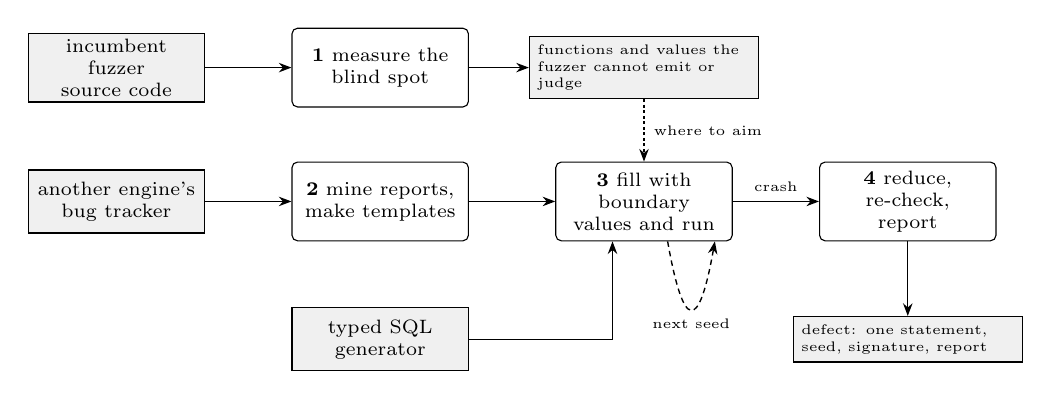
\begin{tikzpicture}[
    x=1cm, y=1cm, font=\scriptsize,
    box/.style={draw, rounded corners=2pt, align=center, inner sep=2pt,
                minimum height=10mm, text width=21mm, fill=white},
    src/.style={draw, align=center, inner sep=2pt, fill=black!6,
                minimum height=8mm, text width=21mm},
    outbox/.style={draw, align=left, inner sep=3pt, fill=black!6,
                text width=27mm, font=\tiny},
    flow/.style={-{Stealth[length=1.6mm]}, line width=0.5pt},
    hint/.style={-{Stealth[length=1.6mm]}, line width=0.5pt, dash pattern=on 1pt off 1pt},
    back/.style={-{Stealth[length=1.6mm]}, line width=0.5pt, dash pattern=on 2pt off 1.5pt},
  ]
  % inputs
  \node[src] (fz)  at (0, 1.7)  {incumbent fuzzer\\source code};
  \node[src] (trk) at (0, 0)    {another engine's\\bug tracker};
  \node[src] (gen) at (3.35,-1.75) {typed SQL\\generator};
  % steps
  \node[box] (s1) at (3.35, 1.7) {\textbf{1} measure the\\blind spot};
  \node[box] (s2) at (3.35, 0)   {\textbf{2} mine reports,\\make templates};
  \node[box] (s3) at (6.7, 0)    {\textbf{3} fill with boundary\\values and run};
  \node[box] (s4) at (10.05, 0)  {\textbf{4} reduce, re-check,\\report};
  % outputs
  \node[outbox] (o1) at (6.7, 1.7) {functions and values the\\fuzzer cannot emit or judge};
  \node[outbox] (o4) at (10.05,-1.75) {defect: one statement,\\seed, signature, report};
  % edges
  \draw[flow] (fz) -- (s1);
  \draw[flow] (s1) -- (o1);
  \draw[flow] (trk) -- (s2);
  \draw[flow] (s2) -- (s3);
  \draw[flow] (gen.east) -| ([xshift=-4mm]s3.south);
  \draw[hint] (o1) -- node[right, font=\tiny] {where to aim} (s3);
  \draw[flow] (s3) -- node[above, font=\tiny] {crash} (s4);
  \draw[flow] (s4) -- (o4);
  \draw[back] ([xshift=3mm]s3.south) to[out=-80, in=-100, looseness=5]
        node[below, font=\tiny] {next seed} ([xshift=9mm]s3.south);
\end{tikzpicture}

  \caption{Workflow of \tool. Step~1 runs once and tells Step~3 where to aim.
  Steps~2 and~3 supply two sources of statements, mined templates and a typed
  generator. Step~3 loops over seeds and is the only step whose cost grows with
  the budget; a crash goes to Step~4.}
  \label{fig:overview}
\end{figure*}

\subsection{Step 1: Measure the Blind Spot}
\label{sec:step-blind}
We read the incumbent fuzzer's source and extract three facts: (i)~its function
vocabulary \Voc; (ii)~its literal domain \Lit; and (iii)~its reference engine
\Rengine. For Turso these are a table of 47 scalar functions and a default literal
policy in two source files~\cite{tursofuzzer}. The policy sets
\texttt{int\_max} to 1{,}000{,}000 and restricts strings to alphanumeric
characters of at most 50 bytes. Every function outside \Voc, every integer outside
the range, every non-alphanumeric string, and every function SQLite lacks is in
\Blind by Equation~\eqref{eq:blind}. This step takes reading, not running. It
needs no new tool, and we do not claim reading source code as new. What we
claim is that this reading should come first.

\subsection{Step 2: Mine Reports and Make Templates}
\label{sec:step-mine}
\tool collects closed issues that carry the tracker's label for a confirmed
defect; for DuckDB this label is \emph{reproduced}. For each issue it fetches the
fixing commit and the regression test that the fix added, and extracts every SQL
statement from that test and from the issue body. Setup statements such as
\sql{CREATE TABLE} and \sql{INSERT} are kept with their query, so a reproduction
brings its own schema and data.

Each extracted query becomes a template. \tool replaces every literal with a
hole typed by the literal's kind (integer, real or string) and leaves everything
else exactly as written: function names, nesting, clauses and setup.
Figure~\ref{fig:motivating}b shows the result for one query. We keep the
structure fixed on purpose. Re-pointing a mined query at a new schema would need
column types and arities to match, and a wrong substitution produces SQL that
merely looks plausible. A query whose structure is unchanged is valid by
construction, so no repair step is needed. The cost is that \tool cannot explore
a structure that no report contains.

\subsection{Step 3: Fill with Boundary Values and Run}
\label{sec:step-run}
\tool fills each hole from a pool weighted toward the edges of each type. For
integers the pool holds zero, $\pm 1$, the limits of 8-, 16- and 32-bit integers,
and the limits of 64-bit integers, including \imax. String holes are filled from
a pool of short ASCII strings. Every random choice comes from a generator seeded
per case, and the seed is stored with each result.

Mined templates are one source of statements. The second is a typed SQL generator
that builds a schema, inserts rows, and composes expressions and queries. It
emits only features that the target engine accepted when \tool probed it, so it
rarely wastes a case on syntax the engine rejects. Its string pool also includes
multi-byte values such as \sql{'é'} and three-byte Chinese characters. A command
line flag selects either source or both.

Each case, meaning its setup statements and its query, runs in a fresh
\texttt{tursodb} process under a time limit and a memory limit. The crash oracle
classifies the outcome into one of six classes (\emph{none}, \emph{user error},
\emph{internal error}, \emph{panic}, \emph{crash}, \emph{timeout}) and reports
only the last four. We do not claim the crash oracle as new; fuzzers have used it
for decades. We chose it because it is the one oracle that can judge a function
the reference engine lacks.

\subsection{Step 4: Reduce, Re-check and Report}
\label{sec:step-triage}
A violation is not yet a finding. \tool groups violations by a \emph{signature},
a hash of the oracle, the error class and the error text with numbers and paths
removed. It then (i)~reduces the statement while keeping the same violation;
(ii)~re-runs it on a fresh process and on a build of the current upstream main
branch, so that a defect fixed last week is not reported; (iii)~searches the
upstream tracker and records the queries it used; and (iv)~drafts a report. A
person reads the draft, reproduces it, and decides whether to file it. Reduction
by repeated deletion is standard and we do not claim it as new. The duplicate
check matters more than it looks. In our campaign it withheld one candidate,
because an upstream pull request had already changed the code it touched.

\section{Implementation}
\label{sec:impl}

\tool is written in Python~3.14 in 10{,}034 lines across 38 files, grouped
into five packages: engine adapters, the corpus pipeline, the typed generator,
the oracle, and triage. It depends on four libraries: PyYAML for configuration,
requests for the GitHub API, sqlglot for reducing statements that parse, and
pytest. A suite of 514 tests (5{,}041 lines) passes in about 31 seconds. Two
problems we met while building it are worth reporting, because both produced
wrong results that looked like right ones.

\paragraph{Errors arrive in the middle of results.} \tool drives
\texttt{tursodb} as a subprocess rather than through a library binding. The
defects we look for end the process, and an in-process binding would take the
test harness down with it. The cost is a text protocol. Turso writes errors to
standard output, interleaved with result rows. Our first adapter looked for an
error only on the first line of the output. A query that returned two rows and
then failed therefore came back as three rows of data, the third being the error
message. The adapter now scans the whole output, and a regression test covers
this case.

\paragraph{A declared type is not a stored type.} The generator first assumed
that if \sql{CREATE TABLE t(c DATE)} parsed, the engine supported dates. SQLite
and Turso map any unknown type name to a storage class, so such a column really
holds integers. A generator built on that assumption reports type coverage it
does not have. \tool therefore probes the real binary once, records which types
it can tell apart and which functions exist, and refuses to emit anything else.

\paragraph{The seed is the state.} Every random choice comes from a seeded
generator, and a campaign writes its last seed on every progress report. A
campaign can stop and resume exactly, and any single case can be regenerated
from its seed alone. Section~\ref{sec:rq1} uses this to regenerate each defect.

\section{Evaluation}
\label{sec:eval}

We ask four questions.
\begin{itemize}
  \item[\rqref{1}] Does \tool find previously unknown defects in an engine that
        already fuzzes itself, and are they accepted upstream?
  \item[\rqref{2}] At an equal budget, which defects does each source of
        statements reach: mined templates, the typed generator, or both?
  \item[\rqref{3}] Do the defects lie in the blind spot of the engine's own
        fuzzers, or could those fuzzers have found them with more time?
  \item[\rqref{4}] What does \tool cost in time and in requests?
\end{itemize}

\subsection{Subjects}
\label{sec:subjects}
We test one engine and mine one other. We chose the engine under test with the
following criteria:
\begin{enumerate}
  \item it is actively maintained and reviews outside contributions, so a report
        gets an answer within weeks;
  \item it can be built from source at any commit, so a defect can be confirmed
        on the current main branch and shown fixed afterwards;
  \item it already runs its own fuzzers, so a defect we find is one those fuzzers
        missed rather than one nobody looked for.
\end{enumerate}
Turso meets all three. We used version 0.9.0-pre.2 at four commits: 730017f96,
where the first campaign ran; b588fbdc6, the last commit before our fixes;
ec86571642a6, which has only our first patch; and 7f0a9e6f4, which has both.
We mined DuckDB because it labels confirmed issues and because its fixes usually
carry a regression test with the triggering query~\cite{duckdb27846}. From 600
closed issues \tool kept 200, and from those it extracted 659 reproductions: 526
from regression tests and 133 from issue bodies.

\subsection{Baselines}
\label{sec:baselines}
\begin{description}
  \item[Mined only.] \tool with templates from DuckDB reports and no generator.
  \item[Generated only.] \tool with the typed generator and no templates. This is
        the plain baseline: a grammar-based fuzzer with boundary values.
  \item[Both.] Each case is drawn from either source.
  \item[Turso's own fuzzers.] Not run by us. We read their source to answer
        \rqref{3}.
\end{description}
All three runs use the same budget of 20{,}000 cases, the same seeds 0 to
19{,}999, the same crash oracle, and the same binary, b588fbdc6, which has none
of our patches.

\subsection{Measurements}
\begin{description}
  \item[\rqref{1}.] Defects found, their upstream state, the exit status and
        output of each reduced statement before and after our patches, and
        whether the tool regenerates each one from a single seed.
  \item[\rqref{2}.] Per run: cases executed, the share the engine accepted, oracle
        hits, and distinct signatures, with the first seed that reaches each.
        The same runs repeated on the build with only our first patch.
  \item[\rqref{3}.] For each defect, whether its function is in Turso's fuzzer
        vocabulary, whether its literals are in that fuzzer's domain, and whether
        SQLite implements the function.
  \item[\rqref{4}.] Wall-clock time and cases per second for each run, and
        requests made to build the corpus.
\end{description}

\subsection{Setup}
All measurements ran on one laptop: an Intel Core i7-1360P with 16 logical CPUs
and 15\,GB of memory, under Linux kernel 7.0, with Python 3.14.4 and Rust
1.88.0. Each case had a 10-second time limit. The statement for defect~4 also ran
under a 6\,GB memory limit, so the pre-fix build would fail fast instead of
building a string of several gigabytes. Each run in Section~\ref{sec:rq2} was
done once; Section~\ref{sec:threats} discusses what that allows us to claim.

\subsection{\rqref{1}: Does \tool Find New Defects?}
\label{sec:rq1}

\begin{table*}[t]
  \caption{The four defects, each run as one statement in a fresh process.
  \emph{Before}: Turso b588fbdc6, which has none of our patches.
  \emph{After}: 7f0a9e6f4, which has both. Exit status 134 is SIGABRT.
  \emph{Found by}: how the defect was first found. \emph{Seed}: the seed that
  makes \tool regenerate the defect in a single case in the run that draws from
  both sources. Defect~4 ran under a 6\,GB memory limit;
  3{,}999{,}999{,}996 is $10^9$ characters times 4 bytes, minus the
  one-character input.}
  \label{tab:defects}
  \footnotesize
  \begin{tabular}{@{}rllrrll@{}}
    \toprule
     & Function & Defect & Before & After & Found by & Seed \\
    \midrule
    1 & \sql{lpad}   & allocates before the length check & 134, 2.28\,s & 1, 0.02\,s & \tool & 4{,}553 \\
    2 & \sql{rpad}   & allocates before the length check & 134, 2.24\,s & 1, 0.02\,s & \tool & 101 \\
    3 & \sql{repeat} & allocates first; size can overflow & 134, 2.27\,s & 1, 0.02\,s & \tool & 5{,}080 \\
    4 & \sql{lpad}   & counts characters, limit is bytes & 134, 3.96\,s & 1, 0.02\,s & review of our patch & -- \\
    \bottomrule
  \end{tabular}
\end{table*}

Table~\ref{tab:defects} lists the defects. Defects 1 to 3 share a cause:
\sql{lpad}, \sql{rpad} and \sql{repeat} sized their result from the caller's
argument and allocated it before comparing it with
\texttt{Value::MAX\_BLOB\_LENGTH}. At a length near \imax the allocation fails and
Rust aborts the process before the check, which ran only on the finished
result, is reached. \sql{lpad} and \sql{rpad} share one function body,
\texttt{pad()}, so defects 1 and 2 have one root cause. We count them separately
because each aborts the engine on its own, and a user who calls only \sql{rpad}
is exposed. \sql{repeat} is a separate function that also multiplies, so its fix
needed an overflow check as well. \tool found all three: the first abort came
eight seconds into the first campaign. One patch fixed
them~\cite{turso11219,turso11225}.

Defect 4 became reachable only after that patch, and \tool did not find it. With
the check now running first, it compared a count of characters with a limit in
bytes. A four-byte fill such as an emoji passes a check of $10^9$ characters, and
about 4\,GB is built before the byte limit rejects it. We noticed the unit
mismatch while writing the first patch, but our pull request described it as
``conservative'', meaning harmless. Turso's automated reviewer replied that it
was permissive and supplied a demonstrating input. We then diagnosed the root
cause, and a second patch computes the exact byte length before building
anything~\cite{turso11260,turso11259}. On a debug build without a memory limit,
the statement ran for about 34 seconds and peaked at 11.7\,GB.

\begin{observation}
\label{obs:found}
\tool found three previously unknown defects in Turso, each of which ends the
process from one statement. Fixing them exposed a fourth, which \tool did not
find. Our two patches, which fix all four, were merged upstream.
\end{observation}

\begin{observation}
\label{obs:seed}
\tool regenerates each of the three defects it found from one recorded seed, in
a single case, on the pre-fix build: seed 4{,}553 for defect 1, 101 for defect 2
and 5{,}080 for defect 3. We checked that each seed calls the function its
defect names.
\end{observation}

\subsection{\rqref{2}: Mined Templates versus Typed Generation}
\label{sec:rq2}

\begin{table*}[t]
  \caption{Each source of statements at an equal budget of 20{,}000 cases and
  seeds 0 to 19{,}999. \emph{Valid}: share of executed cases the engine
  accepted. \emph{Hits}: oracle violations on the pre-fix build. \emph{Distinct}:
  distinct signatures, since eight hits on one signature are one defect found
  eight times. The next three columns give the first seed that reached each
  signature, or a dash if none did. Defects 1 and 2 share a signature; in all
  three runs its first hit was an \sql{rpad} call. The third signature is
  defect~1 again, reached with a length above $10^9$ computed from table data.
  \emph{After patch 1}: hits when the same run is repeated on ec86571642a6, the
  build with only our first patch.}
  \label{tab:ablation}
  \footnotesize
  \begin{tabular}{@{}lrrrrrrrr@{}}
    \toprule
    Source & Executed & Valid & Hits & Distinct & Defects 1, 2 & Defect 3 & Defect 1, second signature & After patch 1 \\
    \midrule
    Mined only     & 19{,}169 &  8.9\% &  8 & 2 & 914 & 10{,}180 & --       & 0 \\
    Generated only & 20{,}000 & 98.3\% & 12 & 3 & 762 & 5{,}367  & 6{,}376  & 0 \\
    Both           & 19{,}759 & 71.1\% & 15 & 3 & 101 & 5{,}080  & 5{,}429  & 0 \\
    \bottomrule
  \end{tabular}
\end{table*}

Table~\ref{tab:ablation} gives the result. Both sources reached both root causes
of defects 1 to 3: the shared \texttt{pad()} body and \sql{repeat}. The generator
reached one more signature. On inspection it is defect~1 again: an \sql{lpad}
call whose length, above $10^9$, is computed from table data. We first took this
signature for defect~4. Repeating every run on the build with only our first
patch settled it: all hits disappear, while that build still aborts on the
defect-4 statement. So no source reached defect~4.

The reason is in the boundary pools. Defect~4 needs a length of at most $10^9$
characters whose result is more than $10^9$ bytes, so between $2.5\times10^8$ and
$10^9$ for a four-byte fill. The integer pools jump from 32{,}767 to
2{,}147{,}483{,}647. None of the 60{,}000 cases that the three modes generate for
seeds 0 to 19{,}999 contains an integer literal in that range. The pools hold the limits of machine integers, not the
limits the engine sets itself.

Mined templates are wasteful but well aimed. Only 8.9\% of their cases ran at all,
because most DuckDB reproductions use syntax Turso rejects. Still, those few
valid cases reached both root causes. Drawing from both sources found the first
defect at seed 101, against 762 and 914 for either source alone, and recorded the
most hits.

\begin{observation}
\label{obs:gen}
At an equal budget, mined templates and typed generation each reached both root
causes of defects 1 to 3. No source reached defect~4, because no boundary pool
holds a length near the engine's own limit of $10^9$.
\end{observation}

\begin{observation}
\label{obs:both}
Drawing from both sources reached the first defect at seed 101, compared with 762
and 914 for each source alone, and recorded 15 hits against 12 and 8.
\end{observation}

\subsection{\rqref{3}: Could Turso's Own Fuzzers Have Found Them?}
\label{sec:rq3}

\begin{table}[t]
  \caption{Why Turso's own fuzzers cannot find the four defects, measured on the
  source at b588fbdc6~\cite{tursofuzzer}. \emph{Voc.}: the function is among the
  47 scalar functions of the differential fuzzer, or among those its four
  libFuzzer targets call. \emph{Dom.}: the defect's literal lies in the fuzzer's
  integer range $[-10^6, 10^6]$ or its alphanumeric string set. \emph{Judge}:
  SQLite implements the function.}
  \label{tab:blind}
  \footnotesize
  \begin{tabular}{@{}rllccc@{}}
    \toprule
     & Function & Literal the defect needs & Voc. & Dom. & Judge \\
    \midrule
    1 & \sql{lpad}   & integer $9.2\times10^{18}$ & \xmark & \xmark & \xmark \\
    2 & \sql{rpad}   & integer $9.2\times10^{18}$ & \xmark & \xmark & \xmark \\
    3 & \sql{repeat} & integer $9.2\times10^{18}$ & \xmark & \xmark & \xmark \\
    4 & \sql{lpad}   & multi-byte fill character  & \xmark & \xmark & \xmark \\
    \bottomrule
  \end{tabular}
\end{table}

Table~\ref{tab:blind} answers the question with three independent checks. The
differential fuzzer's table of 47 scalar functions contains none of
\sql{lpad}, \sql{rpad} or \sql{repeat}. None of its four libFuzzer targets, and
no Rust file under its \texttt{testing} directory, mentions them either. The
functions are covered only by hand-written unit tests with small values. Even if
the functions were added, the default integer range stops at $10^6$, and defects
1 to 3 need a length near \imax. Strings are alphanumeric, and defect~4 needs a
multi-byte character. Finally, SQLite has none of the three functions, so a
differential oracle would have nothing to compare against.

\begin{observation}
\label{obs:blind}
All four defects lie in the blind spot of Turso's own fuzzers on every axis we
checked: the functions are absent from their vocabulary, the required literals
are outside their domain, and the reference engine lacks the functions. More time
would not have found them.
\end{observation}

\subsection{\rqref{4}: What Does \tool Cost?}
\label{sec:rq4}

\begin{table}[t]
  \caption{Cost of each run on the pre-fix build in Table~\ref{tab:ablation}.
  \emph{Time}: wall-clock seconds for the whole run. \emph{Rate}: cases executed
  per second. \emph{First}: the case number of the first oracle hit.}
  \label{tab:cost}
  \footnotesize
  \begin{tabular}{@{}lrrr@{}}
    \toprule
    Source & Time (s) & Rate (cases/s) & First \\
    \midrule
    Mined only     & 378.0 & 50.7 & 914 \\
    Generated only & 388.8 & 51.4 & 762 \\
    Both           & 448.3 & 44.1 & 101 \\
    \bottomrule
  \end{tabular}
\end{table}

Table~\ref{tab:cost} gives the cost of each run. Every run finished in under eight
minutes. Drawing from both sources was the slowest per case and the fastest to a
defect: at 44.1 cases per second, case 101 is reached in about two seconds. We do
not have an explanation for the lower rate, and with one run per source we cannot
tell it apart from noise. Building the corpus took 387 requests to the GitHub API,
354 of them answered from a local cache, and is done once. Step~1 costs reading
time rather than compute. The reducer shrank the case for defect~3 to a single
statement in five executions.

\begin{observation}
\label{obs:cost}
One run of 20{,}000 cases took under eight minutes on a laptop. With both sources,
the first defect appeared at case 101, about two seconds into the run.
\end{observation}

\subsection{Discussion}
\label{sec:discussion}

\paragraph{Is mining bug reports better than generating SQL?} Not on this
target. At the same budget both sources reached the same two root causes
(Observation~\ref{obs:gen}). Mining did two things the generator did not. It
found defects~1 and~3 first in time, before the generator's vocabulary contained
\sql{lpad} or \sql{repeat}; we added those functions to the generator only after
the defects were filed. And it pointed the work at pad functions in the first
place. The fair reading is that each source covers a weakness of the other, which
is why drawing from both
reached a defect soonest (Observation~\ref{obs:both}).

\paragraph{Are the defects in one family really four?} They are four ways for a
user to end the process, each from a different statement, so we count them as
four. They are not four independent mistakes: defects 1 and 2 share one
function body, and defects 1 to 3 share one cause and one patch. Upstream records
them as two issues and two pull requests. We report both counts and say which is
which, so that neither inflates the other.

\paragraph{Would more fuzzing time have found them?} No.
Observation~\ref{obs:blind} is a property of the fuzzer's source, not of its
budget. A generator cannot emit a function outside its vocabulary or a value
outside its domain however long it runs. This is the main practical point of the
paper: the incumbent fuzzer's run time tells nothing about how close it is to
these defects. The same holds for \tool and defect~4:
its pools contain no length in the range that defect needs.

\paragraph{Why did fixing three defects reveal a fourth?} Before the first patch,
the length check ran after the allocation, so its unit did not matter: the
process died first. Once the check ran first, its unit became the thing that
decided the outcome. A
patch is a good place to look for the next defect, since it marks code where the
authors' first understanding was wrong. Our own first understanding of defect~4
was wrong too, and a reviewer corrected it.

\paragraph{Does this work on other engines?} We do not know. The method needs a
second engine with many closed, labelled reports that carry reproductions, and
an engine under test that shares enough of its dialect for some reports to run.
Only 16 of 60 reports that we classified by hand looked transferable to another
engine. Testing other pairs of engines, filling string holes with multi-byte
values, and adding each engine's own limits to the boundary pools we leave for
future work.

\section{Related Work}
\label{sec:related}

\paragraph{Grammar-based SQL generation.} Closest to us is SQLBull, which starts
generation from grammar rules a tester marks as feature-rich, then builds a path
back to the root so that every query contains the rule; it found 63 previously
unknown defects in five engines, all crashes, internal errors or assertion
failures~\cite{liang2026sqlbull}. SQUIRREL keeps mutated SQL valid and guides the search with coverage
feedback~\cite{zhong2020squirrel}. We
share their goal and their kind of oracle, but we choose where to aim differently.
SQLBull aims at deep grammar, a property of the language. We aim at what a
specific incumbent fuzzer cannot express, a property of its source, and we take
the queries from another engine's bug reports rather than from a grammar walk.

\paragraph{Oracles for database engines.} Ternary logic partitioning splits a
query into three partitions whose union must equal the
original~\cite{rigger2020tlp}. Non-optimizing reference engine construction
compares an optimized query with a rewrite the optimizer cannot
touch~\cite{rigger2020norec}. Both find wrong answers that leave the process
running, which a crash oracle cannot see. We use the weaker oracle on purpose:
it needs neither a reference engine nor an equivalent rewrite, so it can judge
\sql{lpad}, which SQLite does not have.

\paragraph{Keeping generated input valid.} Grammar-based whitebox fuzzing lifts
symbolic constraints to tokens so that solved inputs parse~\cite{godefroid2008grammar}.
Fuzzilli mutates an intermediate language in which every program stays
valid~\cite{gross2023fuzzilli}. Repair-driven greybox fuzzing mutates freely and
repairs the result back to valid syntax~\cite{bendrissou2026repair}. Directed
grammar-based generation learns which input structures reach a testing goal
from feedback~\cite{kirschner2025directed}. FuzzNG fuzzes Linux system calls
without hand-written descriptions, and found defects in components that Syzkaller
had covered for years~\cite{bulekov2023fuzzng}. We solve the validity problem
more crudely: we keep a mined query's structure fixed and change only its
literals, and we learn nothing from feedback. FuzzNG's lesson, that a
long-running incumbent fuzzer still leaves reachable defects, holds here too; we
differ in locating those defects by reading the incumbent's source rather than
by reshaping its input space.

\paragraph{Recurring defects.} VulPA writes a known vulnerability as a pattern
and finds other code that breaks it with multi-object typestate
analysis~\cite{cao2025vulpa}. FirmRec builds signatures of known
vulnerabilities from how they are exploited and finds them again in firmware
images~\cite{xiao2024firmrec}. A recent study measures the errors of
recurring-vulnerability detectors on vulnerabilities inherited through reused
code~\cite{cao2025antman}. Another shows that code which looks
like a known vulnerability but is already patched causes many false
alarms~\cite{tan2025fvf}. We share the question these works ask: does a known
defect have siblings? But they answer it statically, within one code base or
across copied code. We answer it dynamically, across two engines that share no
code. Our duplicate check before filing plays the role that a patched-code
filter plays for them, but each of our answers is a statement that either ends
the process or does not, so there is no false alarm to filter.

\paragraph{Learning from patches.} Mystique ports a vulnerability patch from one
branch to another with a language model~\cite{wu2025mystique}, and VicDiff
locates the commit that introduced a vulnerability by comparing patching
patterns~\cite{guo2026vicdiff}. Both reuse what a patch says about a defect. We
reuse what a fix's regression test says about where defects live, and move a
failing input rather than a fix.

\section{Threats to Validity}
\label{sec:threats}

\paragraph{Internal threats.} A harness defect can look like an engine defect.
During development our own adapter once read an error message as a result row
(Section~\ref{sec:impl}). We guarded against this as follows:
\begin{itemize}
  \item every reported statement was re-run by hand on a fresh process, on the
        current upstream main branch, before it was filed;
  \item each defect was confirmed on two builds of the same source tree that
        differ only by our patches, so the patch explains the change;
  \item a test engine with planted defects checks that the oracle fires on a real
        defect and stays silent on a correct engine and on invalid SQL;
  \item every seed in Table~\ref{tab:defects} was run again in a single case and
        reproduced the signature claimed.
\end{itemize}
Attributing a hit to a defect is a second internal threat. We first mapped one
signature to defect~4 by hand, and it was defect~1 reached another way
(Section~\ref{sec:rq2}). Every attribution in this paper was therefore checked
against the build that has only our first patch, which separates defect~4 from
the other three. Each run in Table~\ref{tab:ablation} was done once. Seeds make
a run repeatable on the same code, so the counts there are exact for that code.
The first seed at which a source reaches a defect is one sample and not a rate.
Timings come from one laptop and will differ elsewhere. The claims rest on exit
status and error text, which do not vary between our runs.

\paragraph{External threats.} We tested one engine, mined one other engine, and
all four defects are in one family of string functions in one file. Three share a
cause. Nothing here shows that the method finds defects in another engine, and
Section~\ref{sec:discussion} gives two reasons to doubt that it transfers cheaply:
it needs a rich, labelled tracker, and most mined reports do not run on a
different dialect. The comparison in Table~\ref{tab:ablation} measures \tool as
it stands now. The generator gained \sql{lpad}, \sql{rpad} and \sql{repeat} only
after the first defects were filed, so the table does not say which source would
have found them first at that time.

\paragraph{Construct threats.} We measure the blind spot through one table of
functions, one literal policy and a text search of one source tree. That is a
sound lower bound: a generator cannot emit a function it does not name or a value
outside its configured range. It is not a proof that no other code path in the
project reaches the same statement. We also count defects by signature. A
signature is a hash of the error, so two causes can share one, as defects 1
and~2 do, and one cause can have two, as defect~1 does. For that reason we
decided the count by reading the code, not from signatures. The blind-spot
argument itself was formed after the first defect was found, as an explanation
of why it had survived. We present it as a hypothesis that the evidence
supports, not as the reason the first defect was found.

\section{Conclusion}
\label{sec:conclusion}

A fuzzer cannot test a function it never generates or judge one its reference
engine lacks. Turso fuzzes itself with 41{,}205 lines of Rust in continuous
integration. Yet \sql{select LPAD('a', 9223372036854775807, 'b')} ended its
process. None of its fuzzers ever calls \sql{lpad}, their integers stop at
$10^6$, and SQLite has no \sql{lpad} to compare against.

We presented \tool, which reads an incumbent fuzzer's source to find its blind
spot. It fills that region with the shapes of another engine's bug reports and
with typed generation. It judges results with an oracle that needs no reference
engine. It found three previously unknown defects in Turso and regenerates each
from a recorded seed. Our patch for them exposed a fourth, which \tool did not
find, and our two merged patches fix all four. At an equal budget of 20{,}000
cases, mined reports and typed generation each reached both root causes of the
three defects, and drawing from both found the first defect at case 101. The
fourth defect shows the method's own blind spot: boundary pools built from
machine-integer limits miss the limits an engine sets itself.

\section*{Data Availability}
\label{sec:data}
The replication package accompanies this submission~\cite{graftrepo}. It contains the source of
\tool with its 514 tests; the mined DuckDB corpus with the mining run's own
counters; one page per defect with its reproduction, measured before-and-after,
root cause and, for defects 1 to 3, the regenerating seed; both patches with the
issue and pull-request text as submitted; the raw results behind
Table~\ref{tab:ablation}, including the repeat on the first-patch build; and the
exact Turso commits used. The command \texttt{make reproduce} replays the chain
in Figure~\ref{fig:motivating} and, when both Turso builds are present, runs
defects 1 and 4 before and after the patches.

\section*{Use of Generative AI}
A generative AI assistant, Claude by Anthropic, was used during this project for
help with writing and reviewing code, analysing results, and drafting the
upstream issue reports, the documentation and this paper. Its use is disclosed in
the body of both issues filed with the Turso maintainers. The authors checked
every statement, every citation and every number. Every citation was verified
against its DOI record, and all numbers reported here were produced by running
the tool and the commands given in the replication package.

\section*{Author Contributions}
\label{sec:contributions}

This report is anonymous, as FSE's double-anonymous review requires. The signed
contribution statement, which names each member, states the part of the work
each member led, and carries each member's signature, is therefore kept outside
the report, in the file \texttt{CONTRIBUTIONS.md} of the replication package.
All authors took part in the design, the implementation, the campaigns, the
triage of every candidate and the preparation of both upstream patches, and each
can explain every part of the work.


\bibliographystyle{ACM-Reference-Format}
\bibliography{references}

\end{document}
